

\chapter{Indexology}\label{ch:indexology}
\begin{quote}
... should not prevent us from avoiding purely formal calculations where a \emph{debauchery of indices} hides an often simple geometrical reality. -- E.~Cartan, \emph{Lecons sur la Geometrie des Espaces de Riemann}\sidenote{From Spivak, \emph{A Comprehensive Introduction to Differential Geometry}, volume 2.}\footnote{\cite{spivak1975comprehensive}; see also \url{spivak1975comprehensive}}
\end{quote} % cite https://hsm.stackexchange.com/questions/3320/the-debauch-of-indices-translation-request

In this chapter we introduce the rules for index notation. Please accept them for now as a necessary complication---there is nothing deep here, only a set of conventions and one useful shorthand (summation convention). The utility of these may not be obvious until we start to see how this is used and where it comes from.

\section{Tensors and index notation}
\label{sec:index:notation}

In this course we make a \emph{big deal} about the height of indices. This means the index does more than  `index' a number in an array. In fact, in physics there are objects that carry multiple indices with different heights. Here is one such example, the Riemann tensor in general relativity: $R^a_{\phantom{a}bcd}$. This object has four indices. The first one, $^a$ is raised, and the following three, $_{bcd}$ are lowered. There needs to be an unambiguous ordering of the indices: it is clear that the index $b$ is the \emph{second} index, the index $c$ is the \emph{third} index, and so forth. So it would be disastrous to write $R^a_{bcd}$ because now we cannot tell whether the upper index $^a$ or the lower index $_b$ is the \emph{first} index. This is demonstrated in Figure~\ref{fig:Riemann:tensor:for:indices}.
\begin{marginfigure}%[th]
    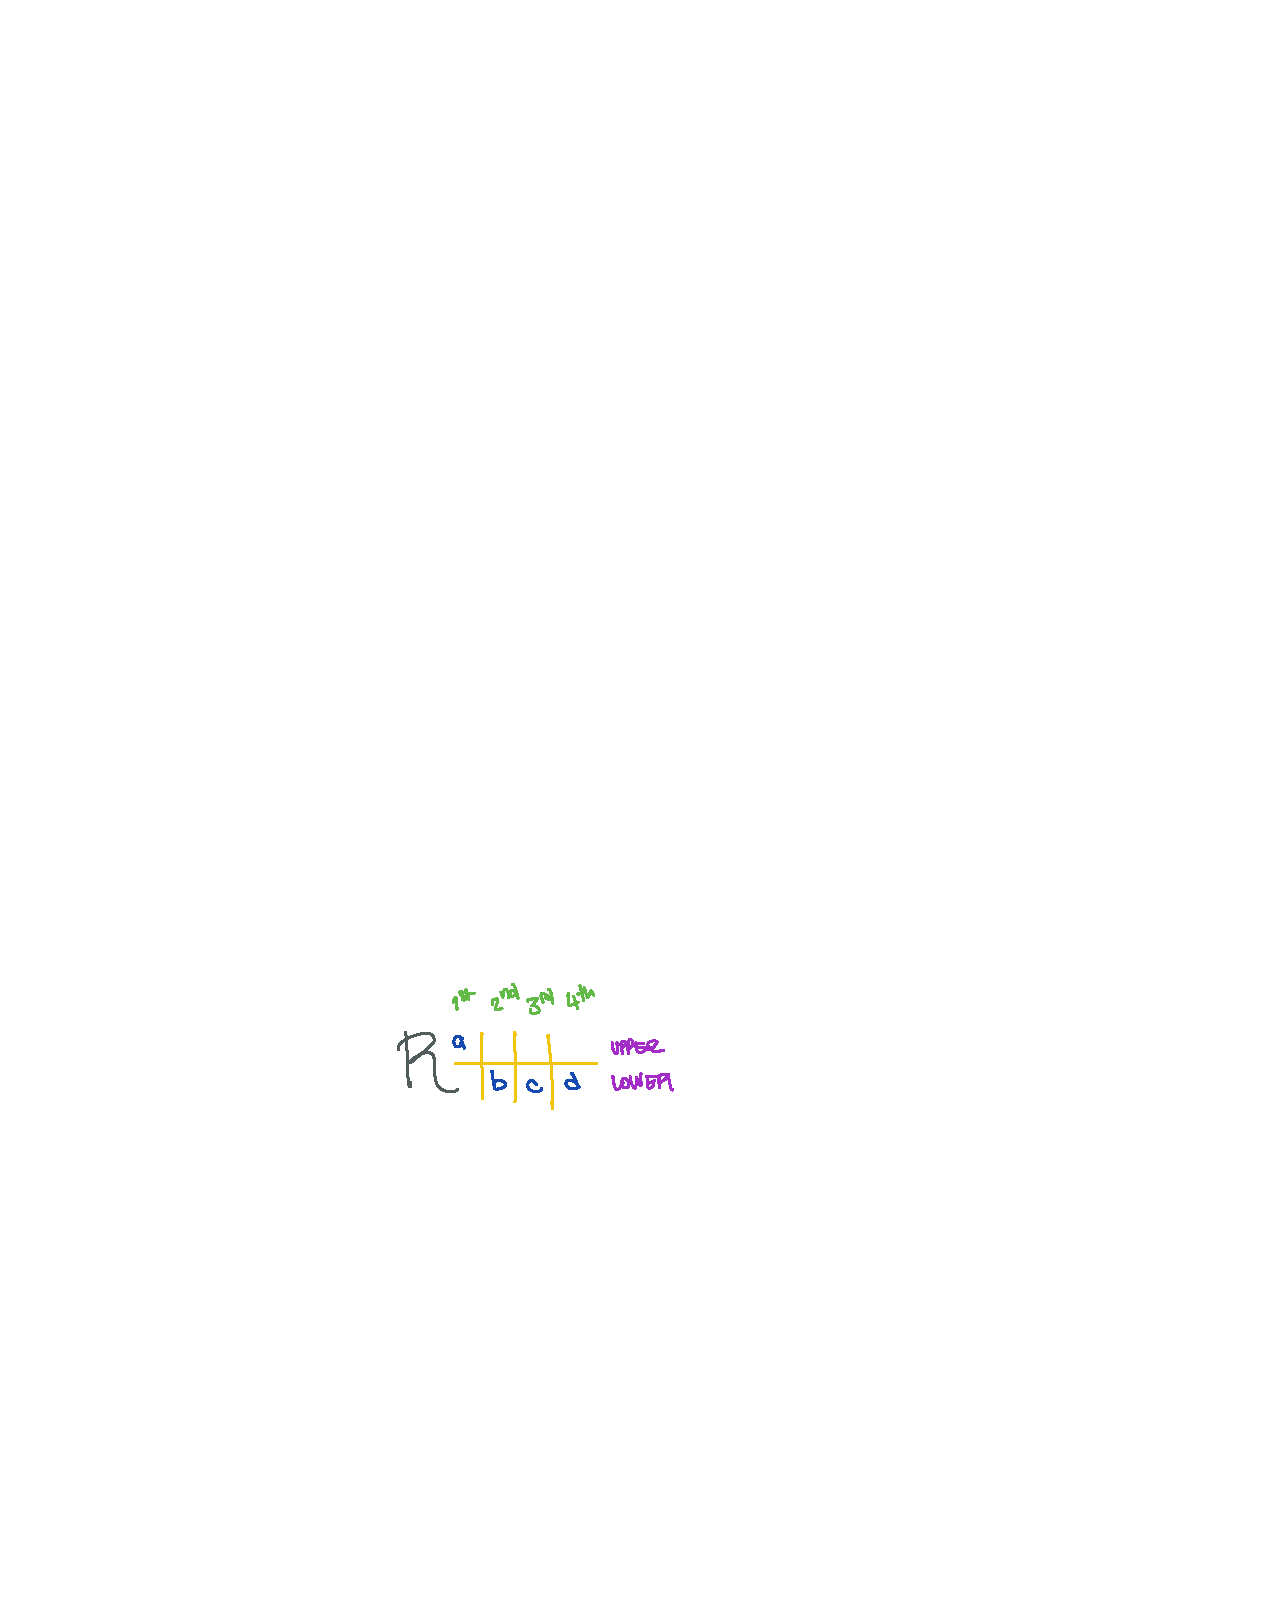
\includegraphics[width=.8\textwidth]{figures/Rabcd_eg.pdf}
    \captionsetup{font={scriptsize,sf}}
    \caption{The Riemann tensor showing the significance of the ordering and height of its indices.}
    \label{fig:Riemann:tensor:for:indices}
\end{marginfigure}

So let us get to the elephant in the room. To a physicist, a \textbf{tensor}\index{tensor} is an object that has indices. In this sense, vectors and matrices are both types of tensors. They can have any number of indices, but the indices have a well defined order and a well defined height (raised or lowered). In general, the following two objects are different:
\begin{align}
    M\aij{i}{j} &&\text{and} && M_i^{\phantom{i}j} \,
\end{align}
even though both are two-index objects whose first index is $i$ and second index is $j$. 

Why do we make such a big deal about indices and their heights? The difference between a tensor and an array of numbers is that tensors have specific \emph{transformation rules} under symmetries. The symmetry that you are most familiar with is rotational symmetry. From your first-year coursework, you are familiar with how useful it is to rotate to coordinates where a problem is simpler. The most common example of this is calculating the moment of inertia of a rotating body. There we had an object called the \emph{moment of inertia tensor}\sidenote{The transformation rules of this tensor are precisely why it is not called a ``moment of inertia \emph{matrix}.'' Though you may be hard pressed to find an honest textbook that explains this.\footnotemark}\footnotetext{See e.g.\,\url{https://hepweb.ucsd.edu/ph110b/110b_notes/node24.html}} One of the groan-inducing exercises in mechanics is to find the rotation in which the moment of inertia tensor of a rotating body is diagonal.

Here is what we need to know for now:
\begin{enumerate}
    \item In physics, tensors are objects with indices. These are arrays of numbers so that a particular choice of indices corresponds to a number in the tensor. The order of the indices matters.
    \item But there is more: whether an index is upper or lower indicates how that part of the tensor transforms under a symmetry transformation such a rotations. 
\end{enumerate}
At this point, you may have several questions, such as these:
\begin{enumerate}
    \item How exactly does a tensor transform under symmetries?
    \item What are examples of other symmetries?
    \item How should I visualize an object with more than two indices? (Yes, you can think of a three-index object as a hypercube arrays of numbers. No, I do not know of a good way to visualize upper versus lower indices on this array.)
\end{enumerate}
We shall answer these as we build up the machinery below. Just take this section as a request to believe that there may be method to this madness.

\section{The treachery of indices}
\label{sec:treachery:of:indices:vi:is:not:a:vector}

There is something that physicists do that tend to drive mathematicians crazy: we write a generic \emph{component of a vector} and refer to it as if it were the vector itself. It is a fairly harmless peccadillo:\sidenote{There are times when you can get into trouble if you drink your own Kool Aid, so to speak. The reason is that the \emph{component} $v^i$ is simply a number, whereas $\vec{v}$ is a vector. Some manipulations are only allowed for numbers and not vectors, and you should be clear that you mean `the component $v^i$' if you are treating it like a number, and not `the \emph{vector} whose components are $v^i$.' %See Example~\ref{eg:moving:coefficients:around}.
} if I say
\begin{quote}
the vector $v^i$
\end{quote}
then it is not hard to guess that I mean
\begin{quote}
the vector $\vec{v}$ which has components that I label $v^i$.
\end{quote}
If you ever meet a mathematician who gives you a hard time about this, you can wave your hands and refer to something called \emph{abstract index notation}, developed by Roger Penrose.\footnote{\url{https://math.stackexchange.com/questions/455478/}} To the best of my understanding, this is simply a formal way to justify the way physicists talk about indices. 

The reason why we have this culture is that this index notation ends up being so damn convenient. In addition to vectors, we will have other objects that have indices: dual vectors, matrices, and tensors. When we write everything in with indices, we can ``see'' properties of these objects that are not obvious without the indices. Specifically, we can see \emph{how an object transforms under symmetries}. In this course, we will focus on \emph{rotations} of vectors and their generalizations. 

Whenever I think about whether $v^i$ means the vector $\vec{v}$ or the $i^\textnormal{th}$ component of that vector, I am reminded of Magritte's ``The Treachery of Images,'' Figure~\ref{fig:Magritte}\footnote{From \url{https://en.wikipedia.org/wiki/The_Treachery_of_Images}, please refer to this page for fair use justification.}
\begin{marginfigure}%[th]
    
\includegraphics[width=.8\textwidth]{figures/MagrittePipe.jpg}
    \captionsetup{font={scriptsize,sf}}
    \caption{``La Trahison des Images'' (``The Treachery of Images'') by Ren\'e Magritte. Owned by \tacro{LACMA}, reproduced here under fair use.}
    \label{fig:Magritte}
\end{marginfigure}
In this image, Magritte shows a painting of a pipe and then writes ``this is not a pipe.'' The implied message is that it is a \emph{painting} of a pipe that we may use to express the \emph{idea} of a pipe.


\section{Summation Convention}
\label{sec:summation}


There is another reason why indices are convenient: they allow us to use \textbf{summation convention}.\sidenote{Sometimes called Einstein summation convention in deference to its progenitor. With respect to Einstein, we simply write \emph{summation convention} because it's not like the dude is underappreciated in popular culture.} This is a notational shortcut that introduces upper and lower indices to convey sums. Consider, for example, the ``matrix multiplication'' of a row vector $\row{w}$ on a column vector $\vec{v}$. Nevermind the formal definition of ``row vector'' as opposed to ``column vector.'' Let us write it out in components where it is obvious for $\RR ^3$:
\begin{wide}
\begin{align}
    \row{w}
    &=
    \begin{pmatrix}
        w_1 & w_2 & w_3
    \end{pmatrix}
    &
    \vec{v}
    &=
    \begin{pmatrix}
        v^1 \\ v^2 \\ v^3
    \end{pmatrix}
    &
    \row{w}\vec{v}
    &= w_1v^1 + w_2v^2+w_3v^3 \ .
\end{align}
\end{wide}
On the far right we have used the matrix multiplication rules in Section~\ref{sec:matrix:multiplication}.
% The final expression is familiar, right? It follows the usual rules of matrix multiplication for a ``matrix'' that happens to be one row and three columns; 
We review this rule in Fig.~\ref{fig:row:col:mult}, labeling the components with upper and lower indices as appropriate.
% %% FIGURE SNIPPIT
\begin{marginfigure}[.01em]%[tb]
    \centering
    \captionsetup{font={scriptsize,sf}}
    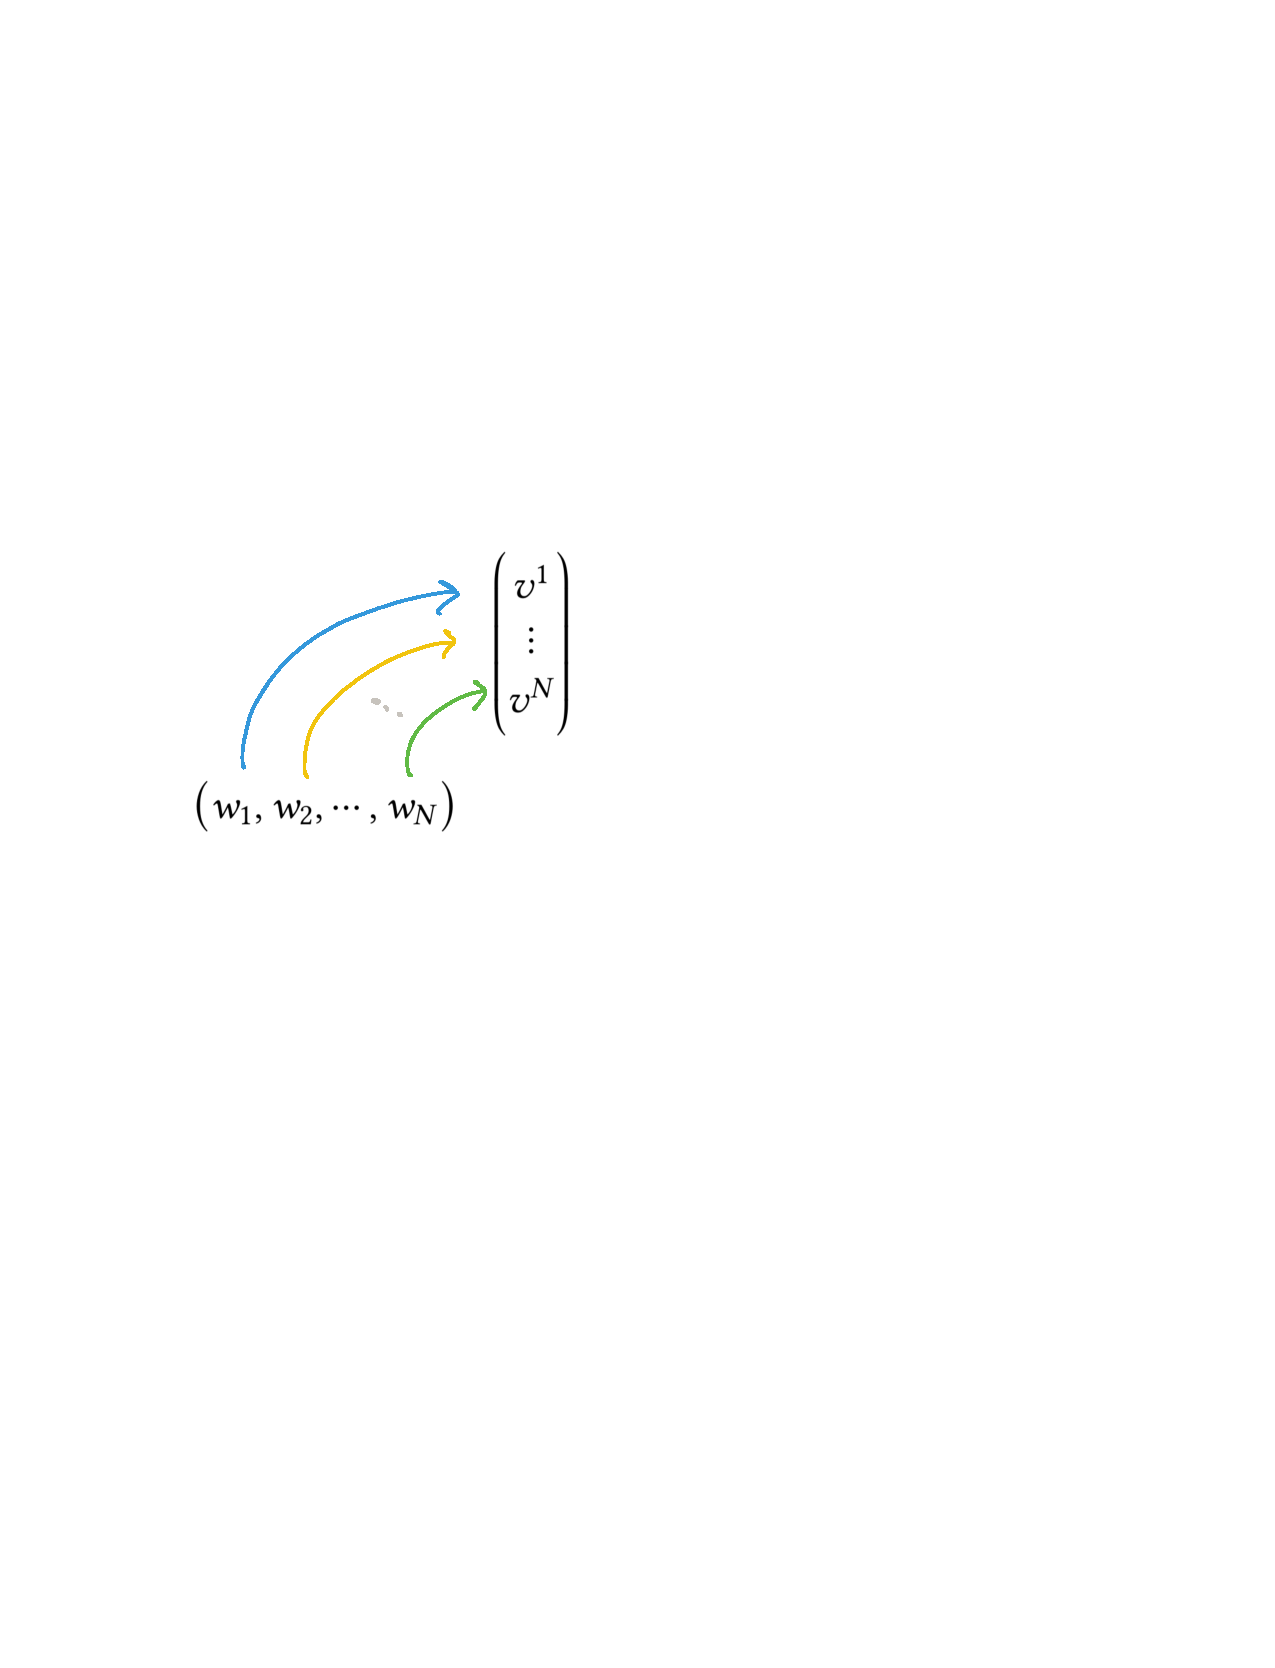
\includegraphics[width=.8\textwidth]{figures/rowcolmult.pdf}
    \caption{The `matrix multiplication rule' for acting with a row vector on a column vector.}
    \label{fig:row:col:mult}
\end{marginfigure}
Notice that we choose to write the components of $\row{w}$ with lower indices---this is the convention. Row vectors have indices written as subscripts while column vectors have indices written as superscripts. There is no mathematics here, just a choice of notation. The result of the multiplication is simply a number, which we can write as a sum:
\begin{align}
    \row{w}\vec{v}
    &= \sum_{i=1}^3 w_iv^i
    \equiv w_iv^i \ .
    \label{eq:row:w:on:vec:v}
\end{align}
On the right-hand side we have \emph{defined} the summation convention:
\begin{newrule}[Summation convention]
Whenever there is exactly one upper index and exactly one lower index with the same letter, we should understand that there is a sum over that index over all of its allowed values. We call pairs of repeated indices where one is upper and one is lower \textbf{contracted indices}\index{contract}.
\end{newrule}



The value $w_iv^i$ is simply a number. It is not a vector. It does not have any ``vectorial'' (tensorial) structure. It is not an element of the vector space $\RR ^3$. It does not transform under rotations. It is \emph{just a number}. In other words, $w_iv^i$ behaves like an object with \emph{no indices}. Contracted indices ``cancel each other out.''

This is significant because we will see that indices tell us how objects transform. Evidently, column vectors and row vectors transform differently since one has an upper index and one has a lower index. Further, when we contract the two indices, we end up with something with no indices: a number that does not transform at all. This may seem like notational overkill---trust me, it is worth building this notation now. We will use it over and over.



\begin{example}
Matrices $M$ have the following index structure: $M\aij{i}{j}$. There is a first index and a second index---the order matters. The first index is upper, and the second index is lower. Matrix multiplication boils down to a contraction of indices:
\begin{align}
    (M\vec{v})^i = M\aij{i}{j}v^j \ .
    \label{eq:matrix:mult:ith:comp}
\end{align}
Let us read this equation carefully. First, $M\vec{v}$ is a vector. The $i^\text{th}$ component of this vector is $(M\vec{v})^i$. How is this related to the components of $M$ and $\vec{v}$? The right-hand side tells us that we simply take the sum:
\begin{align}
    M\aij{i}{j}v^j = 
    M\aij{i}{1}v^1 + M\aij{i}{2}v^2  + M\aij{i}{3}v^3 \ .
\end{align}
\end{example}

\begin{figure}[tb]
    \centering
    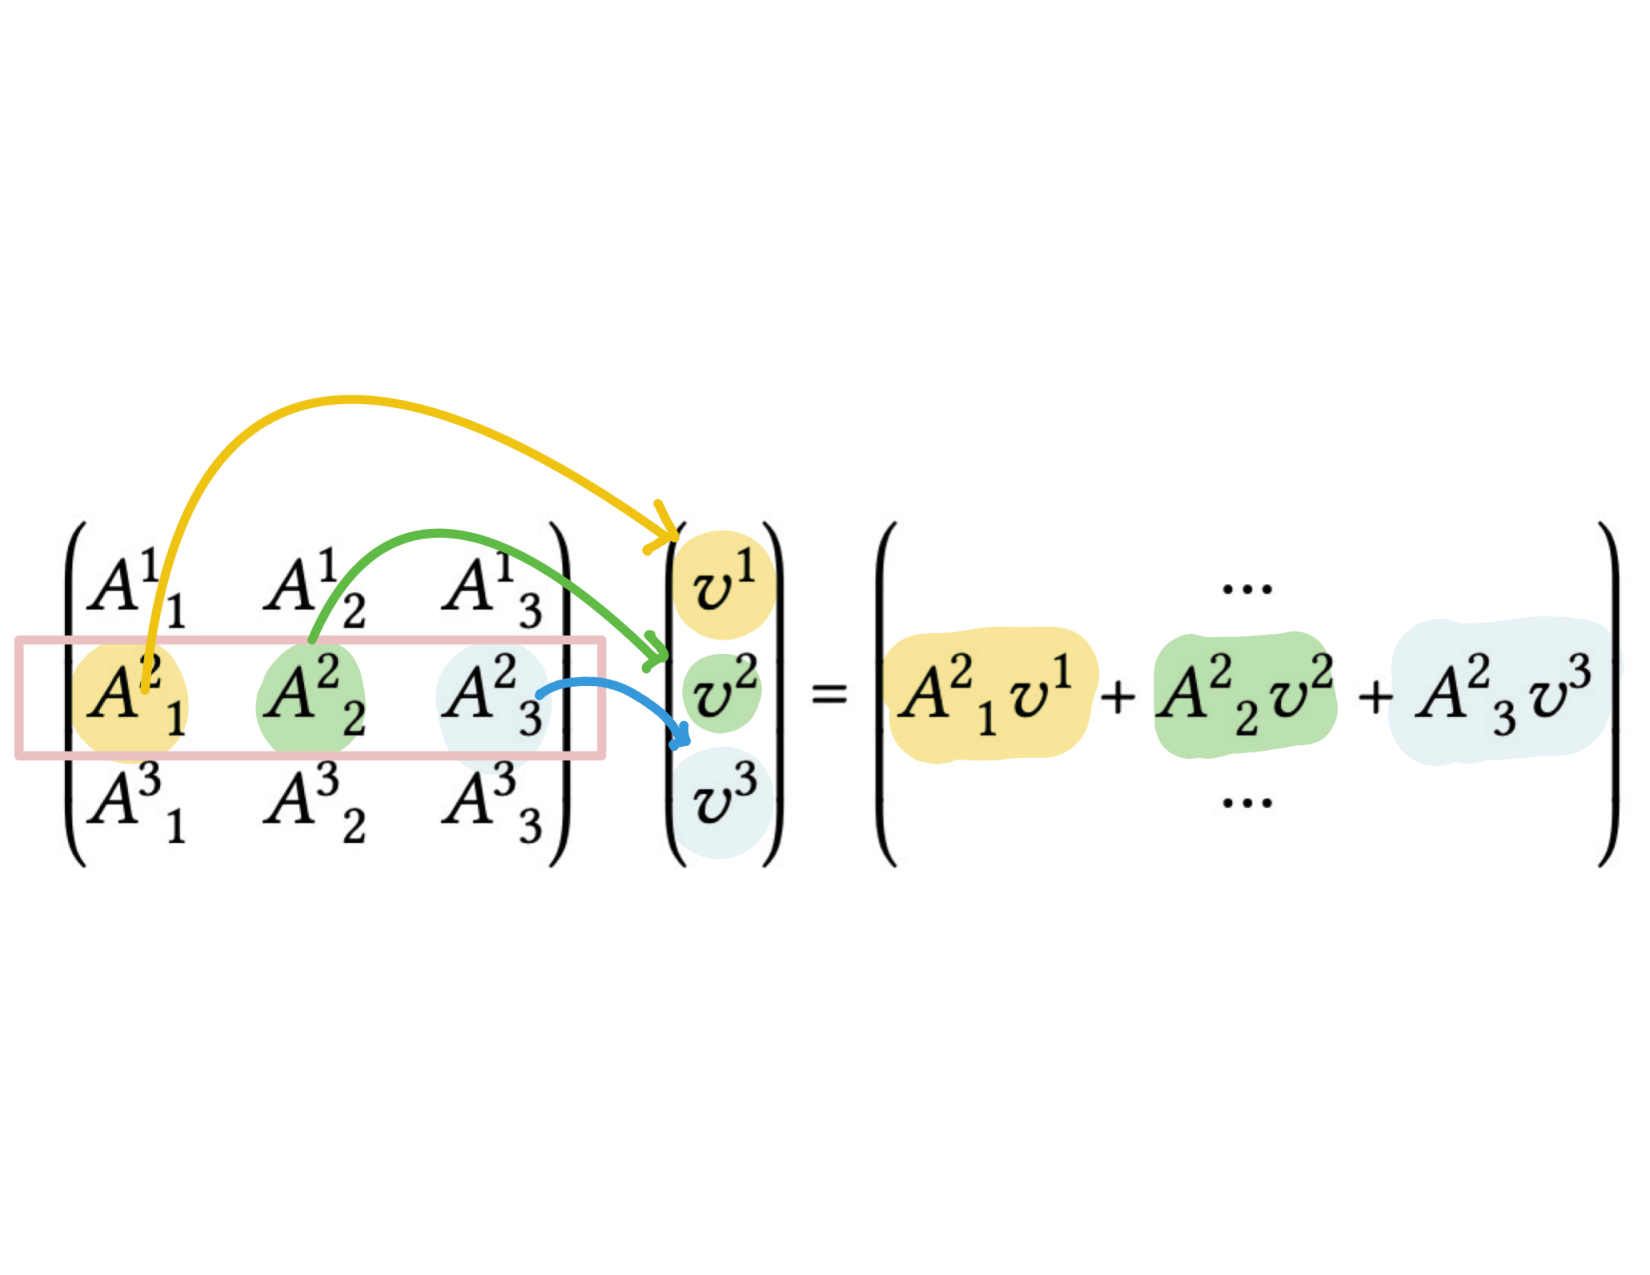
\includegraphics[width=.5\textwidth]{figures/matrixmultiplication.pdf}
    \caption{The `matrix multiplication' rule for $A\vec{v} = \vec{v}'$. We show that the second element of $\vec{v}'$ is a sum of terms, where each term is a multiplication of the $j^\text{th}$ column of the $2^\text{nd}$ row of $A$ by the $j^\text{th}$ row of $\vec{v}$.}
    \label{fig:matrix:col:mult}
\end{figure}

\begin{example}
From the above example, you can then excuse the glib statement: ``the \emph{vector} $M\aij{i}{j}v^j$.'' As we explained above, $M\aij{i}{j}v^j$ is not a vector, but a component of a vector. However, the point is that even though there are three indices, two of them are contracted so the object effectively only has one upper index. This is the index structure of a vector. This matches the usual matrix multiplication rule shown in Fig.~\ref{fig:matrix:col:mult}.
\end{example}

\begin{exercise}
Consider the following vector, row vector, and matrix:
\begin{align}
    \vec{v} &=
    \begin{pmatrix}
     1 \\ 2 \\ 3   
    \end{pmatrix}
    &
    \row{w} &=
    \begin{pmatrix}
        4&5&6
    \end{pmatrix}
    &
    M&=
    \begin{pmatrix}
        1 & 2 & 3 \\
        4 & 5 & 6 \\
        7 & 8 & 9
    \end{pmatrix} \ .
\end{align}
These have index structure $v^i$, $w_i$, and $M\aij{i}{j}$ respectively. Note that the first index of a matrix is the row and the second is the column, thus $M\aij{1}{2} = 2$ while $M\aij{2}{1} = 4$. Calculate the following: $(wM)_2$, $(Mv)^1$, $(MM)\aij{1}{2}$. Here $MM$ is understood to be the square of the matrix $M$, $(M^2)\aij{i}{j} = M\aij{i}{k}M\aij{k}{j}$.
\end{exercise}

\begin{example}\label{eg:moving:coefficients:around}
It should be clear that
\begin{align}
    w_i M\aij{i}{j} = 
    w_1 M\aij{1}{j} + w_2 M\aij{2}{j} + w_3 M\aij{3}{j}
    = 
    M\aij{1}{j}w_1  + M\aij{2}{j}w_2 + M\aij{2}{j}w_2
    =
    M\aij{i}{j}w_i \ .
\end{align}
After all, each of the components $w_i$ and $M\aij{i}{j}$ are simply numbers. However: even though $w_i M\aij{i}{j} = M\aij{i}{j}w_i$, it is \emph{completely incorrect} to say $\row{w}M = M\row{w}$. This is because $\row{w}$ and $M$ are \emph{tensorial} (vector-y) objects. The order of their `multiplication' matters. You can see this from the matrix notation.
\begin{align}
    \row{w}M &= 
    \begin{pmatrix}
        4&5&6
    \end{pmatrix}
    \begin{pmatrix}
        1 & 2 & 3 \\
        4 & 5 & 6 \\
        7 & 8 & 9
    \end{pmatrix}
    &
    M\row{w} &=
    \begin{pmatrix}
        1 & 2 & 3 \\
        4 & 5 & 6 \\
        7 & 8 & 9
    \end{pmatrix}
    \begin{pmatrix}
        4&5&6
    \end{pmatrix} \ .
\end{align}
The first multiplication gives a row vector, as you expect since $(wM)_j$ has one lower index. The second multiplication does not even make sense. What we see is that expressions like $w_i M\aij{i}{j} = M\aij{i}{j}w_i$ are valid as long as you are only talking about the components. The glib ``physicist slang'' of replacing a component by its vector/matrix/tensor can get you into trouble if you have moved components around in a way that is only allowed for numbers, but not vectory-things.
\end{example}

Since the language is now becoming cumbersome, let us define the word \textbf{tensorial} to mean an object with indices. This will replace the phrase ``vectory'' in our notes.




One neat thing about this is that our convention for contracting indices makes it clear that $(Mv)^i$ is a component of a vector: it has one upper index. Similarly, you may recall that the multiplication of matrices $M$ and $N$ proceeds as follows:
\begin{align}
 (MN)\aij{i}{j} = M\aij{i}{k}N\aij{k}{j} \ .
 \label{eq:matrix:matrix:multiplication}    
\end{align}
\begin{exercise}
Confirm that \eqref{eq:matrix:matrix:multiplication} holds for $2\times 2$ matrices.
\end{exercise}
On the right-hand side of \eqref{eq:matrix:matrix:multiplication}, we have one pair of contracted indices $_k^{\phantom{k}k}$, one upper index $^i$, and one lower index $_j$. We thus deduce that this object is a matrix: it has one upper and one lower index. Indeed, the product of two matrices is also a matrix. Our indices and contraction rules tell us what kinds of objects we can produce by contracting indices between them. 

\begin{example}
You may also contract indices within an object. For example, because a matrix has one upper and one lower index, you may contract them together. This is called the \textbf{trace}\index{trace}, $\Tr M = M\aij{i}{i}$. Alternatively, you may remember the trace as the sum of all diagonal elements in a matrix. This corresponds to 
\begin{align}
    M\aij{1}{1} + M\aij{2}{2} + \cdots = M\aij{i}{i} \ ,
\end{align}
where we simply recognize that the summation convention is a shortcut for the `sum of all diagonal elements' rule. The significance of the trace is that as an object with no indices---they're both contracted---it is a pure number. Under rotations, the trace does not change. If you measure something that is the trace of a tensor, it does not matter what coordinate system you are in---you measure the same thing.
\end{example}
